\begin{frame}[t]{Модел на FitzHugh-Nagumo}
  Моделът на FitzHugh-Nagumo се стреми да улесни пресмятането на трансмембранния потенциал за сметка на точността.
  \begin{align*}
    &\dv{v}{t} = v - \frac{v^{3}}{3} - w + I_{\rm{ext}} \\
    &\dv{w}{t} = \frac{1}{c}\left(v + a - bw\right)
  \end{align*}
  Тук $w$ е възвръщаша променлива с цел бавен feedback.
  $I_{\rm{ext}}$ е стимулиращ неврона ток.
  Nagumo съпоставил следната електрическа верига:
\end{frame}

\begin{frame}[t]{Модел на FitzHugh-Nagumo}
  \begin{figure}[htbp!]
    \centering
    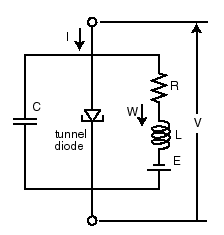
\includegraphics[width=\textwidth,height=0.7\textheight,keepaspectratio]{img/fitzhugh-nagumo/circuit.png}
    \caption{Еквивалентна верига на модела на FitzHugh-Nagumo от Scholarpedia}
  \end{figure}
\end{frame}

\begin{frame}[t]{Модел на FitzHugh-Nagumo}
  \begin{figure}[htbp!]
    \centering
    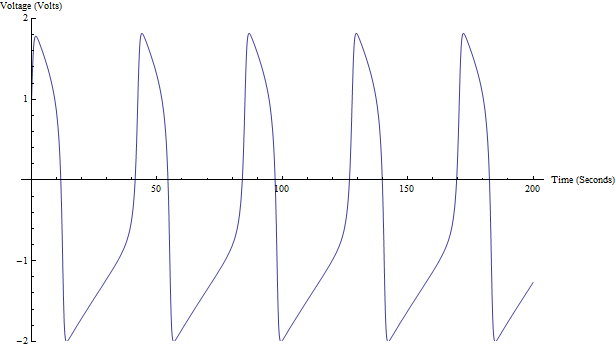
\includegraphics[width=\textwidth,height=0.7\textheight,keepaspectratio]{img/fitzhugh-nagumo/graph.png}
    \caption{Симулация на модела на FitzHugh-Nagumo от Wikipedia}
  \end{figure}
\end{frame}
